\chapter{Experiments}\label{chapter:experiments}
\thispagestyle{chapterBeginStyle}

In this chapter, I will describe the experimental setup with all requires libraries. Section \ref{section:datasets} includes the description, analysis, and examples from the datasets used in the experiments. It also provides an explanation and the assumption on how to simulate a drop in the model performance \ref{remark:performance-drop-while-train} used in training. The model training process is defined in section \ref{section:models}. Because the model performance and training are not a part of experiments, training results are also added to this section. Real-world augmentations used in this study are defined in section \ref{section:augmentation}. These augmentations are applied to the images in the first part of the experiments (described in Section \ref{section:dont-augment-me-definition}). Experiments are divided into two parts. The first part (defined in Section \ref{section:dont-augment-me-definition}) is going to test the effect that augmentations have on attribution methods. The second part (defined in Section \ref{section:can-i-rely-on-you-definition}) is going to check if there is a reliable measurement that can be used to compare XAI methods.

\section*{Environment and framework}

The training environment was designed around the PyTorch library \cite{NEURIPS2019_9015}\footnote{Detailed implementation and guide is available at \url{https://github.com/burnpiro/xai-correlation}, Wiki page with additional instructions and results is available at \url{https://github.com/burnpiro/xai-correlation/wiki}}. Augmentations described in section \ref{section:augmentation} are performed with the help of the G'MIC library \cite{gmic}. Most of the experiments use Captum \cite{kokhlikyan2020captum} and scikit-learn \cite{scikit-learn} libraries to process, analyze and produce results of attribution methods. In the experiments, not all methods are used for all experiments. This is due to the limited amount of memory available on the graphic card used to perform analysis. Methods like Integrated Gradients \cite{sundararajan2017axiomatic} cannot be used to calculate the value of Sensitivity \cite{yeh2019fidelity} because it requires storing over $500$ interpolations to generate the result. These details will be explained in sections describing a particular experiment. All the experiments are run on the \textit{GeForce GTX 1080 Ti} with 11GB of memory, and the total processing time of all experiments is around 508 hours (this assumes running a version with example generation).

\section{Datasets}\label{section:datasets}

All the datasets used in this study are publicly available. The selection process was aimed at finding a variety of different domains and complexity. Five datasets were selected, and each dataset is split into a training dataset and test dataset. If not defined in the dataset description, the split was done using $80:20$ proportions (\textit{training : test}). Besides the original split, each training dataset was additionally split into five training datasets. The second split creates the following structure for every dataset:

\begin{table}[ht]
\centering
\caption{Default dataset split structure}
\label{tab:dataset-split}
\begin{tabular}{|l|l|l|}
\hline
  & Training     & Test \\ \hline
A & 100\% * 80\% & 20\% \\ \hline
B & 80\% * 80\%  & 20\% \\ \hline
C & 60\% * 80\%  & 20\% \\ \hline
D & 40\% * 80\%  & 20\% \\ \hline
E & 20\% * 80\%  & 20\% \\ \hline
\end{tabular}
\end{table}

Table \ref{tab:dataset-split} can be read as \textit{"split B of the dataset X uses 80\% training dataset which consists of 80\% of the entire dataset, and full test dataset which consists of 20\% of the total dataset"}. If the class distribution is not constant, then splits of the train datasets are stratified. 

\begin{remark}\label{remark:performance-drop-while-train}
This split assumes that using a fraction of the training dataset for training will cause models to perform worse when tested on the same test dataset. It should simulate real-world issues with model accuracy and allow to experiment on none perfect models. The drop in the accuracy is not going to be linear because of the different complexities of each data domain.
\end{remark}

\subsection{Stanford Dogs}

The dataset created by Stanford University consists of dog pictures. It has 120 classes, and the train/test data split is defined by the authors. Class distribution is proportional between train and test splits. Dataset is slightly unbalanced, with the ratio between the least frequently occurring class and the most common class being $1.7$ (detailed class distribution available in appendix \ref{appendix:datasets:stanford-dogs}). The total number of images is 20580 (train: 16418, test: 4162). Examples from the datasets can be seen in Figure \ref{fig:stanford-dogs-example}.

\begin{figure}[ht]
    \centering
    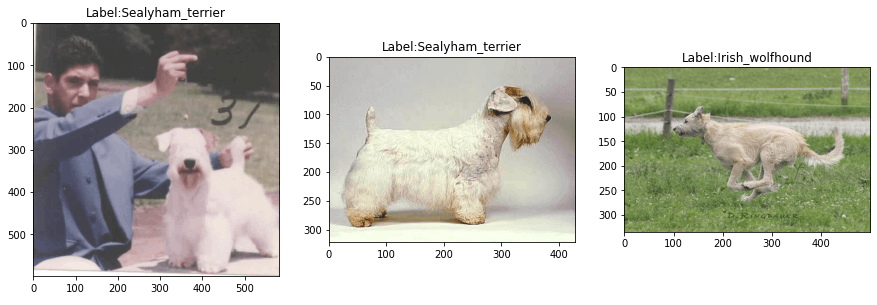
\includegraphics[width=0.65\textwidth]{experiments/datasets/dogs.png}
    \caption{Example images from in \textit{Stanford Dogs} \cite{stanford-dogs}}\label{fig:stanford-dogs-example}
\end{figure}

\subsection{Food 101}

The dataset consists of food pictures. It has 101 classes, and the train/test data split is defined by the authors. Classes are distributed proportionally, and each class has 750 examples in the train dataset and 250 examples in the test dataset, with the total number of images at 101000 (train: 75750, test: 25250). Examples from the datasets can be seen in Figure \ref{fig:food101-example}.

\begin{figure}[ht]
    \centering
    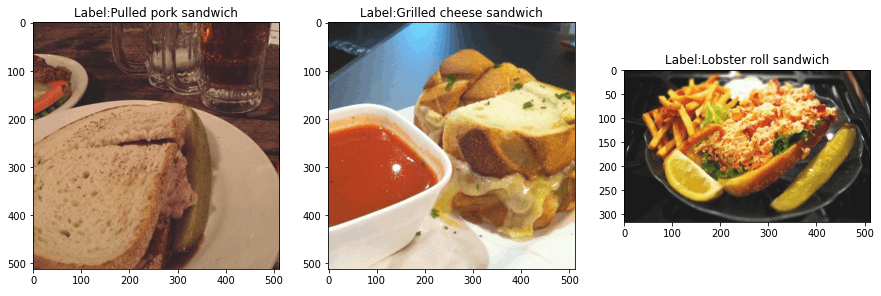
\includegraphics[width=0.65\textwidth]{experiments/datasets/food101.png}
    \caption{Example images from in \textit{Food 101} \cite{food101}}\label{fig:food101-example}
\end{figure}

\subsection{Edible wild plants}

The dataset consists of edible wild plants pictures. It has 62 classes, and the train/test data split is defined by the authors. Class distribution differs between train and test splits. Train dataset is highly unbalanced, with the ratio between the least frequently occurring class and the most common class being $21$ (detailed class distribution available in appendix \ref{appendix:datasets:edible-plants}). The unbalance is caused by 3 major classes. The rest of the dataset has the same ratio equal to $3$. The test dataset is balanced with $5$ examples for each class. The total number of images is 6868 (train: 6558, test: 310). Examples from the datasets can be seen in Figure \ref{fig:edible-plants-example}.

\begin{figure}[ht]
    \centering
    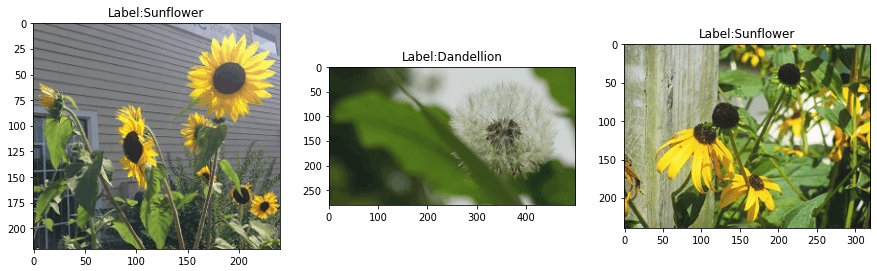
\includegraphics[width=0.65\textwidth]{experiments/datasets/wild-plants.png}
    \caption{Example images from in \textit{Edible wild plants} \cite{edible-wild-plants}}\label{fig:edible-plants-example}
\end{figure}

\subsection{Marvel Heroes}

The dataset consists of pictures from the Marvel Universe franchise. It has 8 classes, and the train/test data split is defined by the authors. Class distribution is proportional between train and test splits. Dataset is fairly balanced with ratio between the least frequently occurring class and the most common class being $1.12$ (detailed class distribution available in appendix \ref{appendix:datasets:marvel}). The total number of images is 3035 (train: 2584, test: 451). Examples from the datasets can be seen in Figure \ref{fig:marvel-example}.

\begin{figure}[ht]
    \centering
    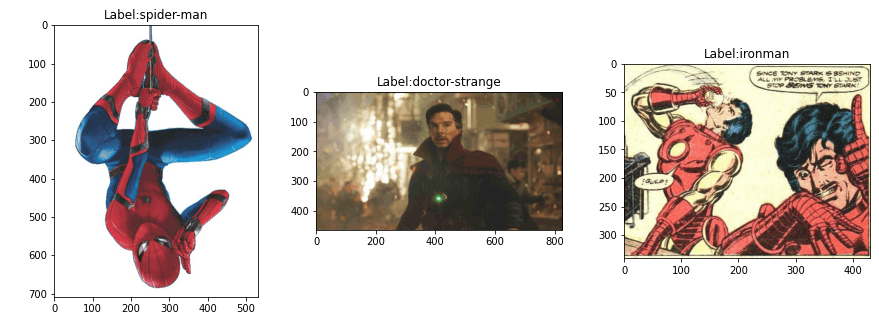
\includegraphics[width=0.65\textwidth]{experiments/datasets/marvel.png}
    \caption{Example images from in \textit{Marvel} \cite{marvel-heroes}}\label{fig:marvel-example}
\end{figure}

\subsection{Plants}

The dataset consists of plant pictures. It has 99 classes, and the train/test data split is defined by the authors. Class distribution is proportional between train and test splits (with the test dataset being slightly more balanced). Dataset is balanced with ratio between the least frequently occurring class and the most common class, being $7$ (detailed class distribution available in appendix \ref{appendix:datasets:plants}). The total number of images is 14670 (train: 13149, test: 1521). Examples from the datasets can be seen in Figure \ref{fig:plants-example}.

\begin{figure}[ht]
    \centering
    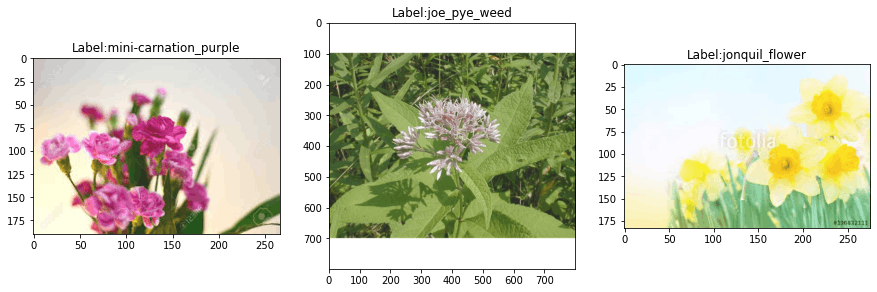
\includegraphics[width=0.65\textwidth]{experiments/datasets/plants.png}
    \caption{Example images from in \textit{Plants} \cite{plants-dataset}}\label{fig:plants-example}
\end{figure}
\section{Models and training}\label{section:models}

This study uses three different model architectures: ResNet 18 \cite{he2015deep}, DenseNet 121 \cite{huang2017densely} and EfficientNet B0 \cite{tan2019efficientnet}. These architectures were selected base on popularity in the data science community and  their availability in popular frameworks. Each model was first pretrained on the ImageNet dataset \cite{imagenet2009}, and fully connected layers from the top of the architecture were removed. There were no further changes to the original structures. On top of the model, a single fully-connected layer was added with the output size matching the number of classes in the particular dataset used for fine-tuning. Fine-tuning is done using Stochastic Gradient Descent (SGD) with momentum \cite{rumelhart1986learning} and Cross-Entropy loss function. Each model was trained for 15 epochs with a decrease of the learning rate (from \textit{0.001} to \textit{0.0001}) after the 7th epoch. Each architecture was trained on every available dataset and every training fraction split of that dataset (train dataset splitting described in section \ref{section:datasets}). In total, $75$ different models were trained for the purpose of the experiments.

\begin{figure}[h]
  \centering
 \begin{subfigure}{.45\textwidth}
    \centering
    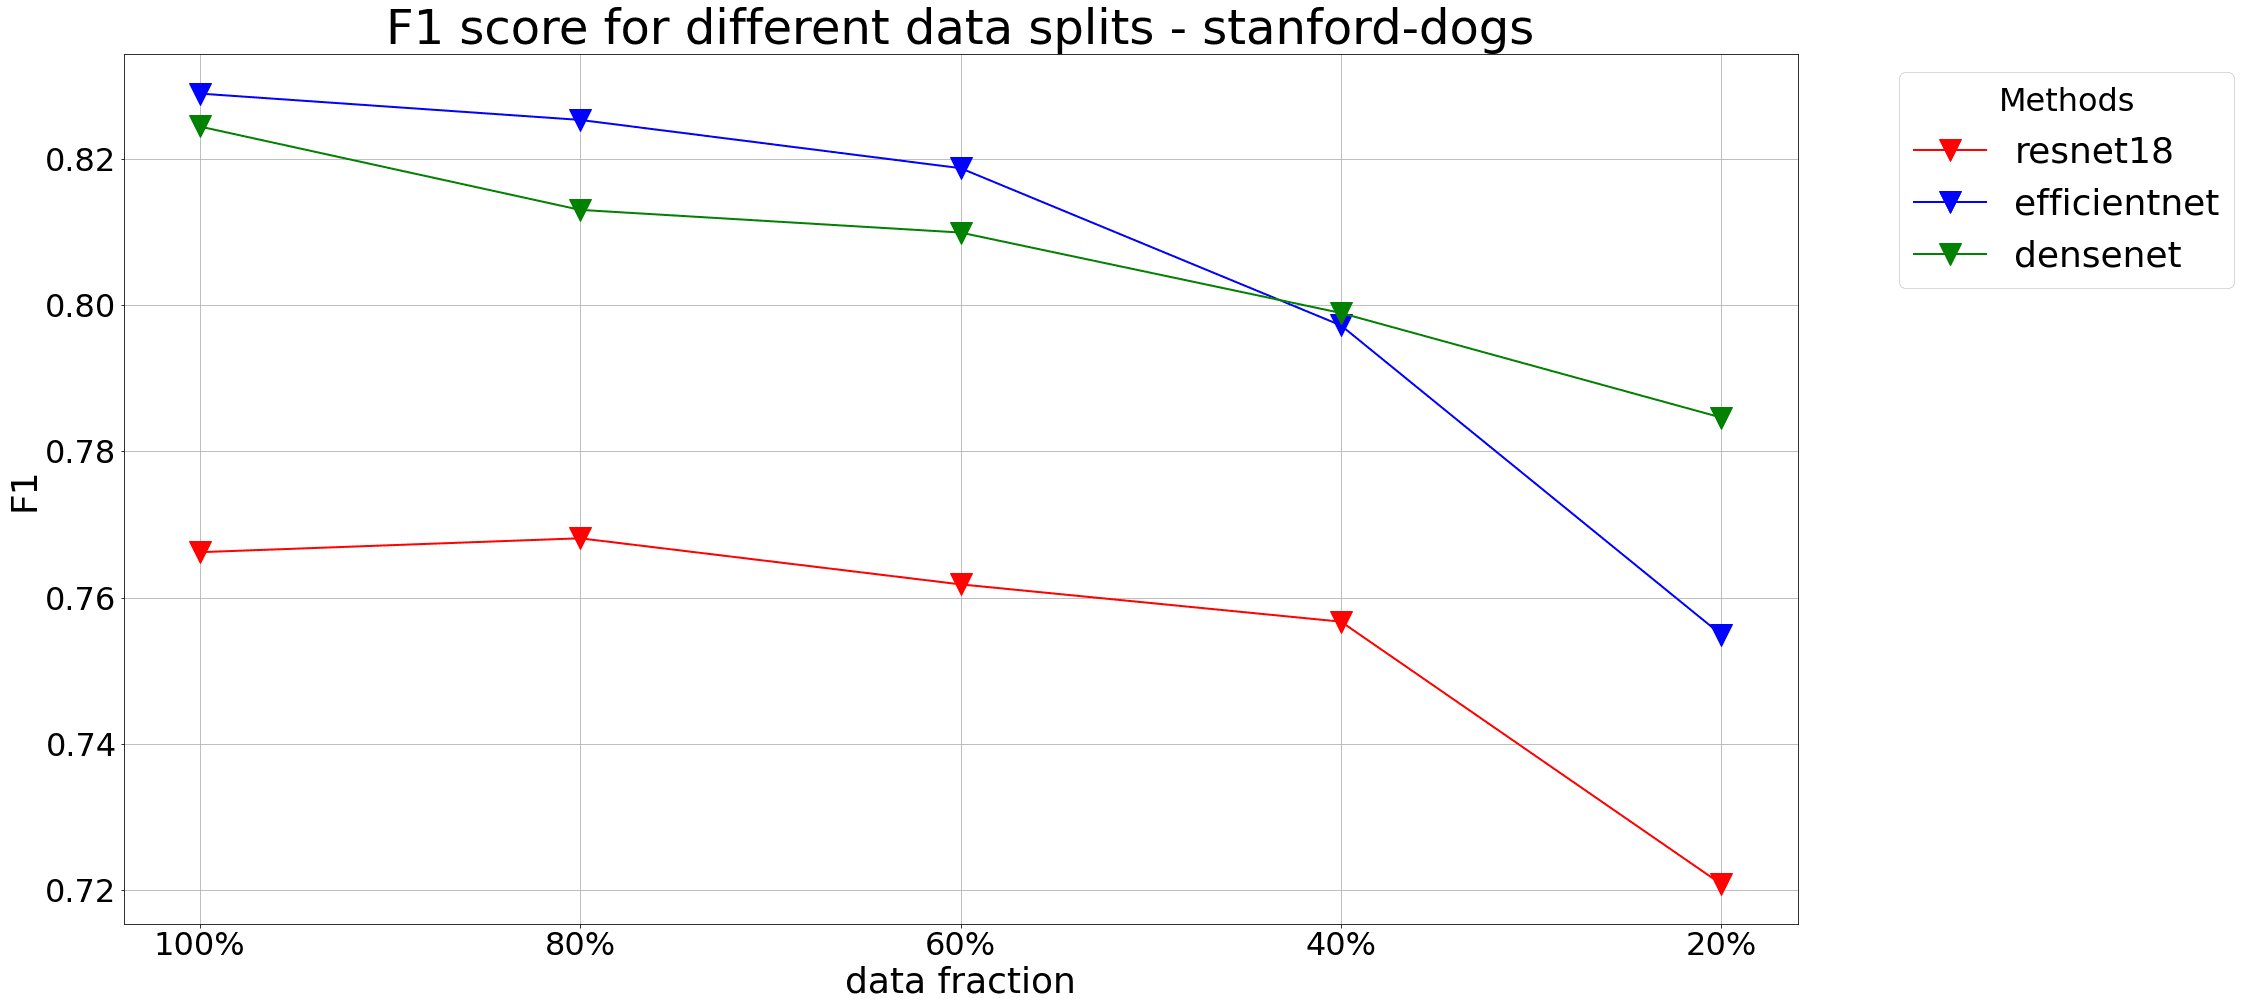
\includegraphics[width=\textwidth]{experiments/models/stanford-dogs-f1.png}
    \caption{Stanford Dogs dataset, F1 scores}\label{fig:model-scores-dogs}
\end{subfigure}
 \begin{subfigure}{.45\textwidth}
    \centering
    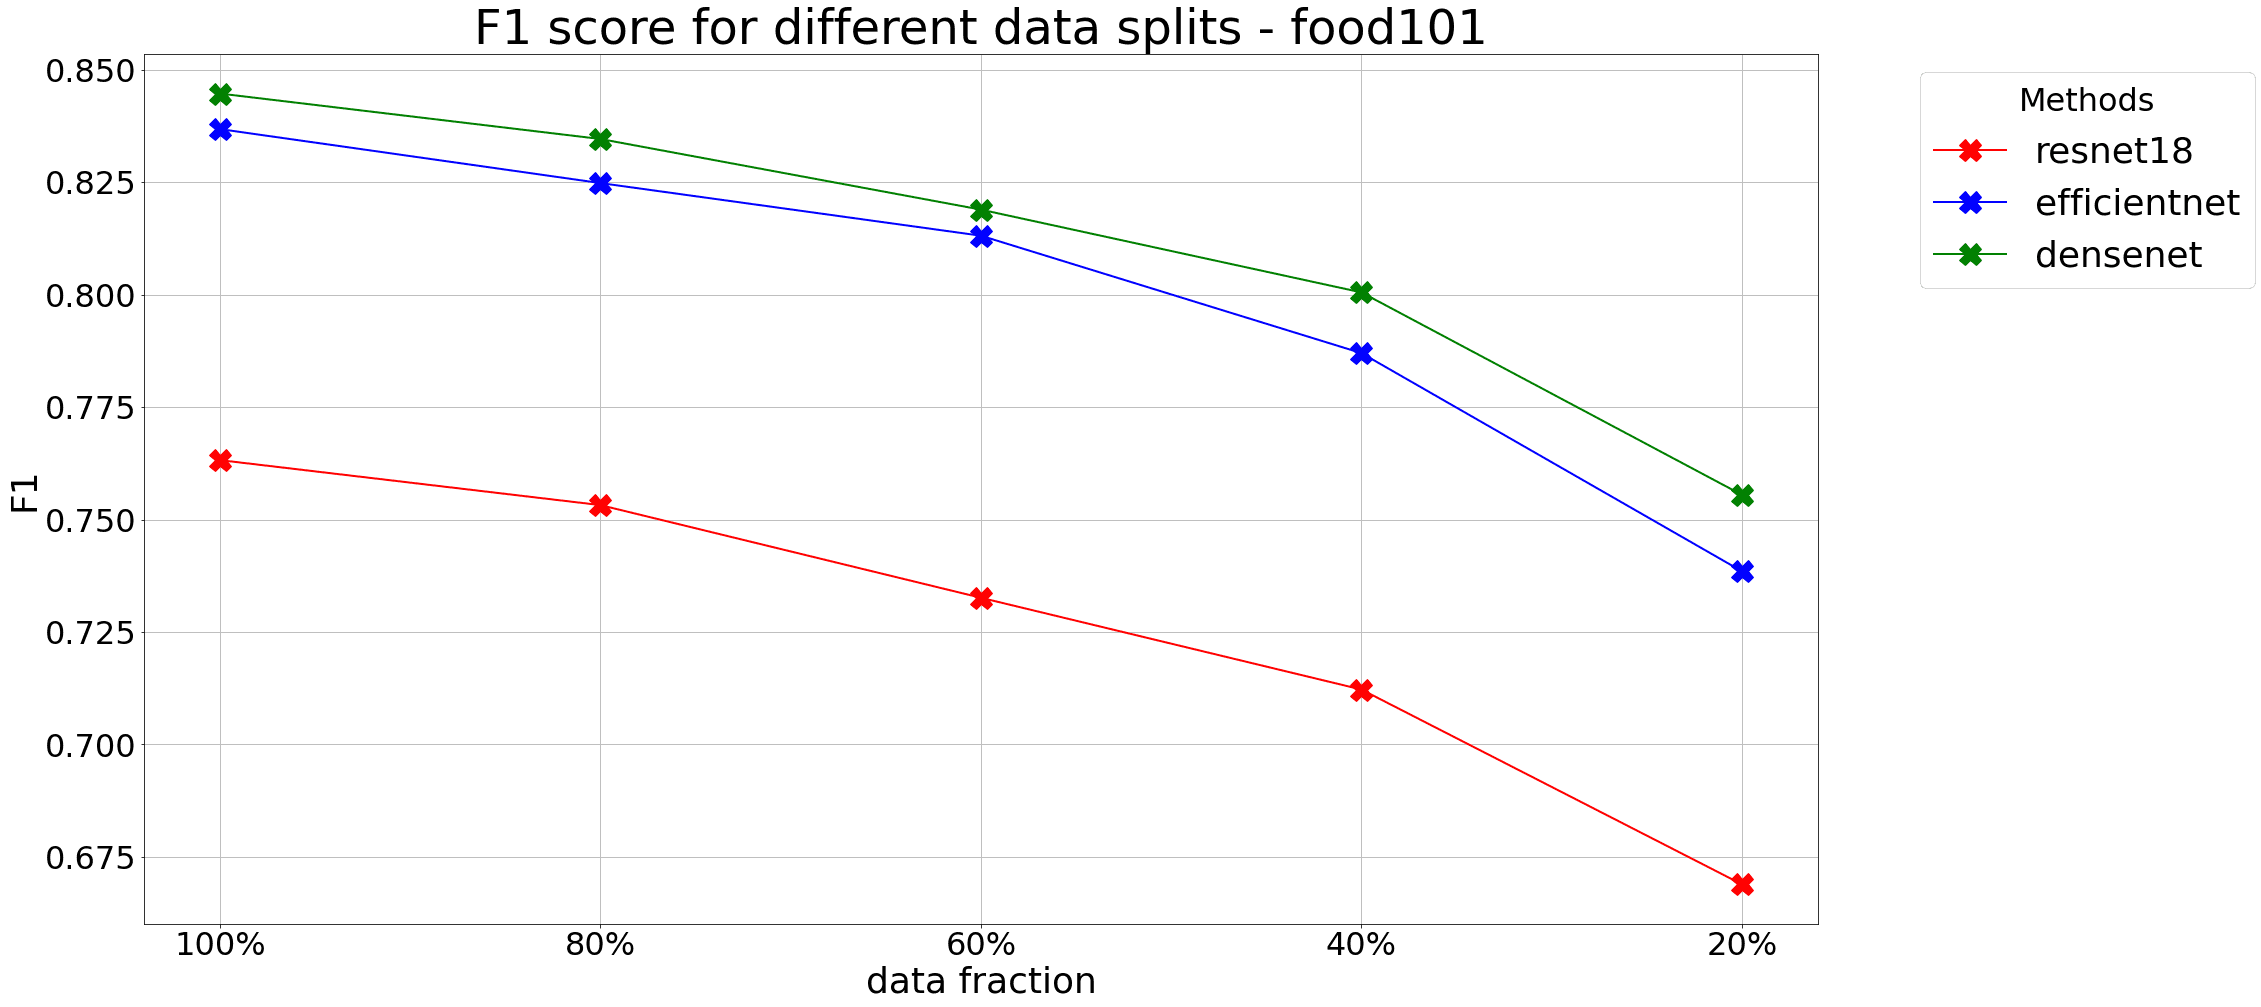
\includegraphics[width=\textwidth]{experiments/models/food101-f1.png}
    \caption{Food 101 dataset, F1 scores}\label{fig:model-scores-food101}
\end{subfigure}
 \begin{subfigure}{.45\textwidth}
    \centering
    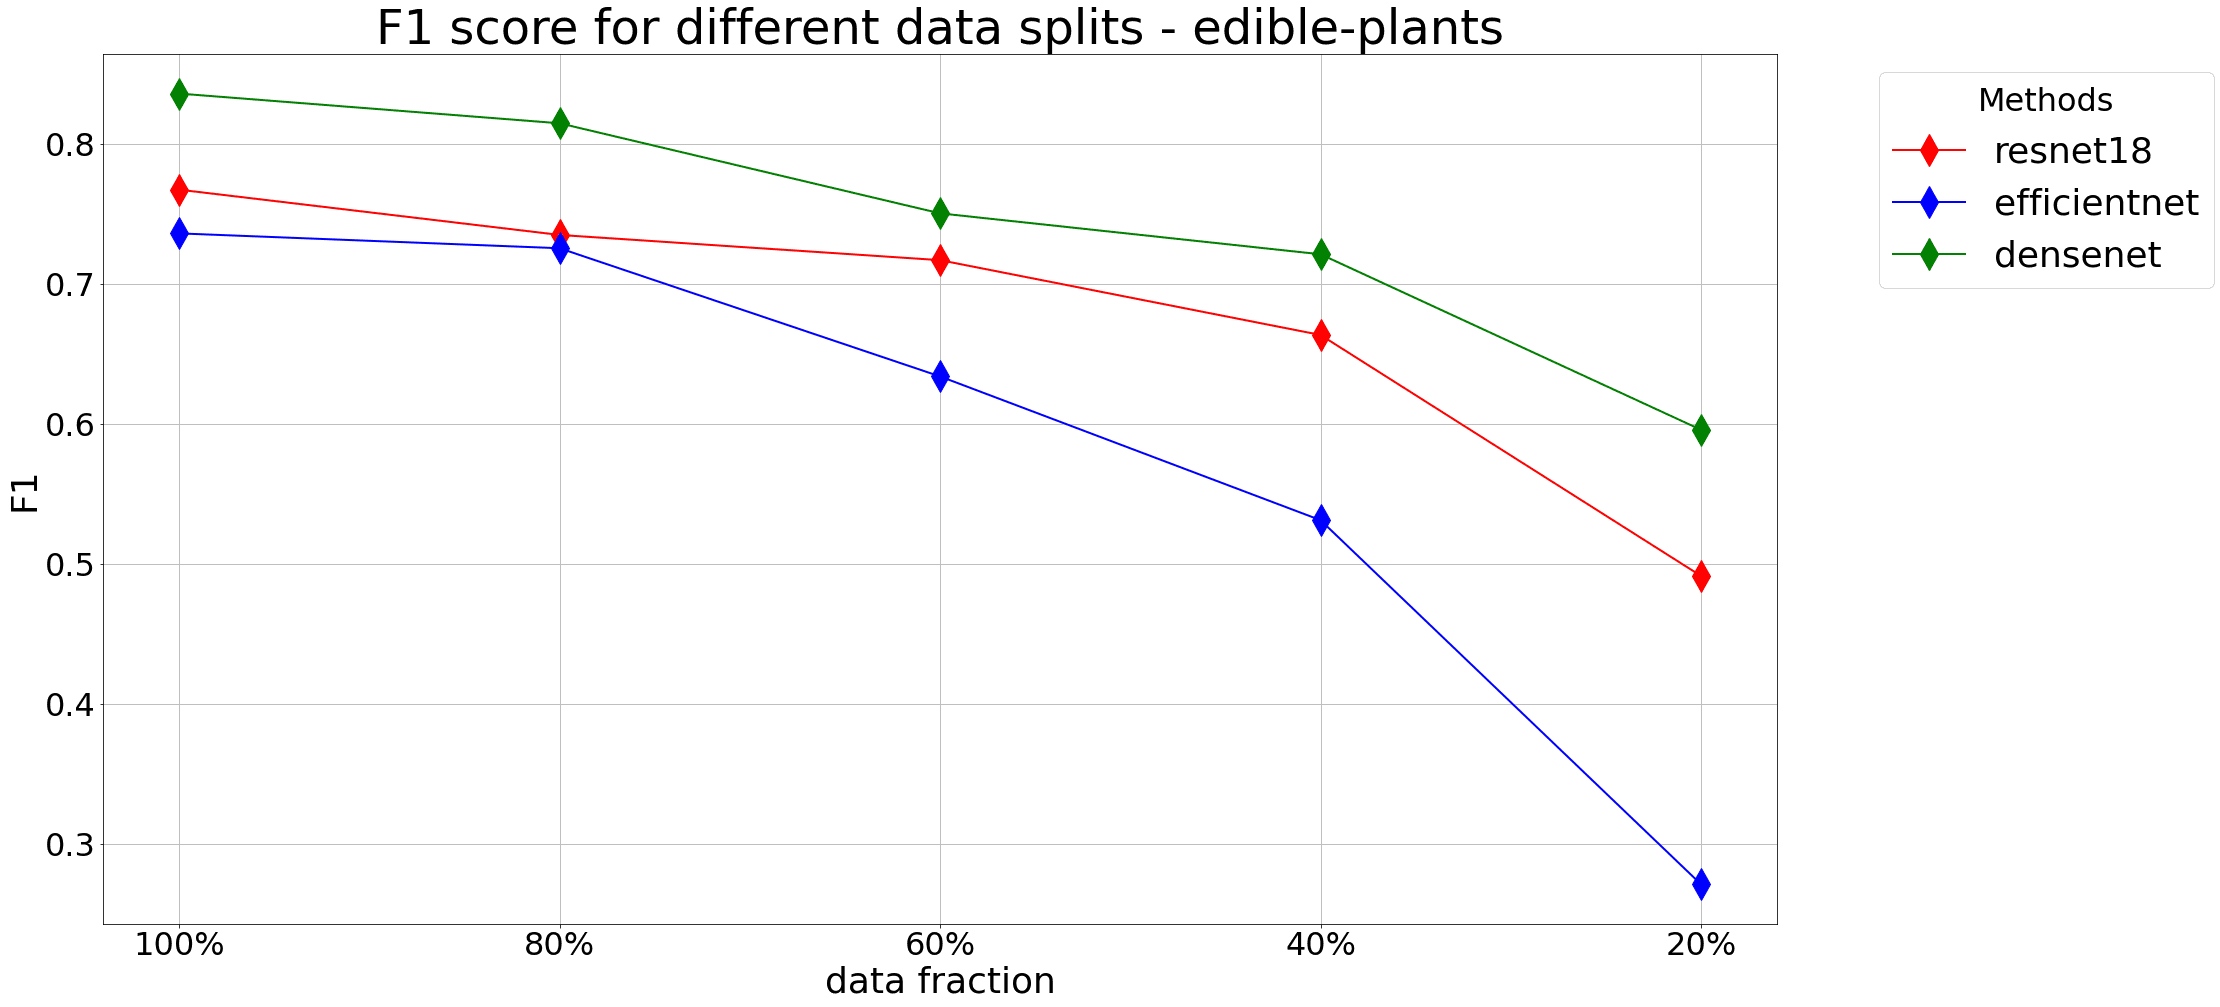
\includegraphics[width=\textwidth]{experiments/models/edible-plants-f1.png}
    \caption{Edible wild plants dataset, F1 scores}\label{fig:model-scores-edible-plants}
\end{subfigure}
 \begin{subfigure}{.45\textwidth}
    \centering
    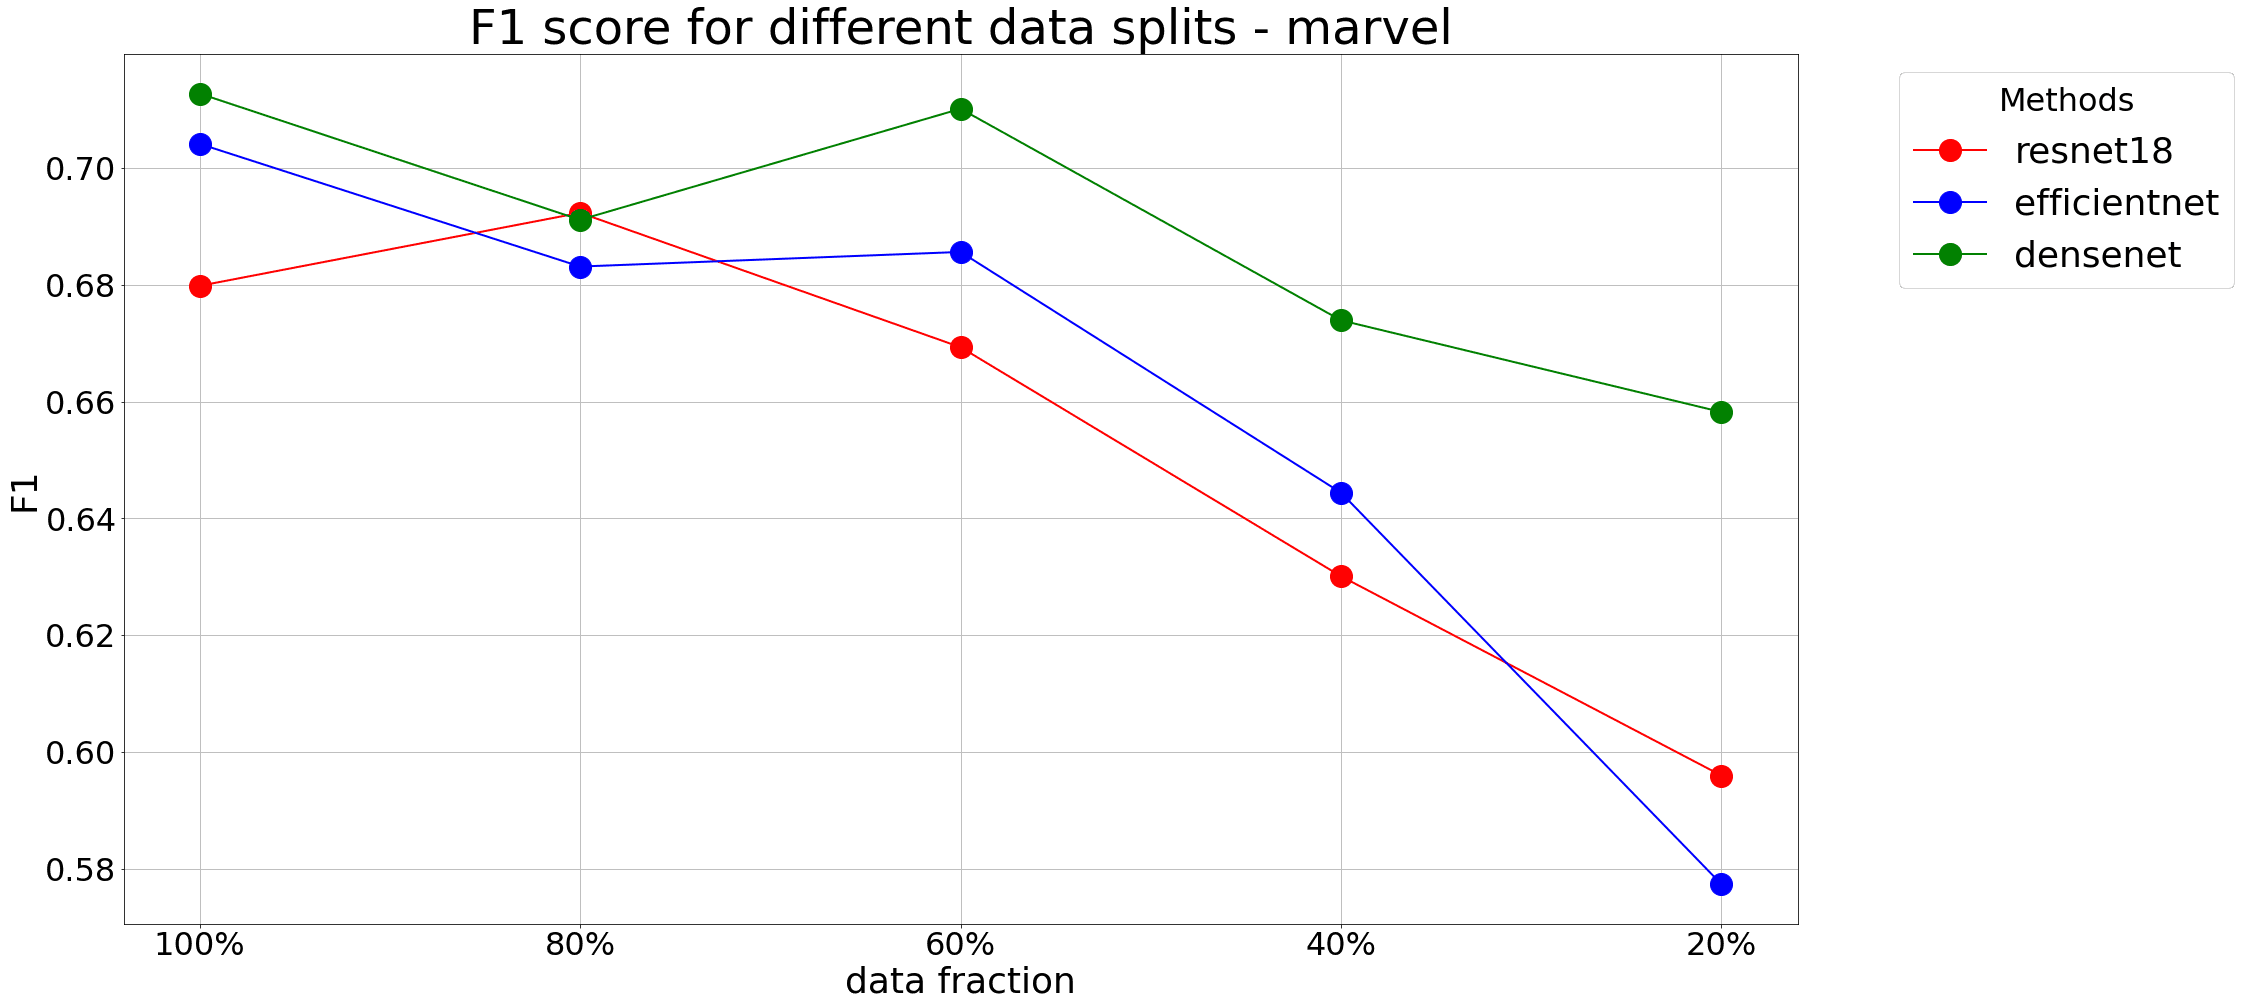
\includegraphics[width=\textwidth]{experiments/models/marvel-f1.png}
    \caption{Marvel dataset, F1 scores}\label{fig:model-scores-marvel}
\end{subfigure}
 \begin{subfigure}{.45\textwidth}
    \centering
    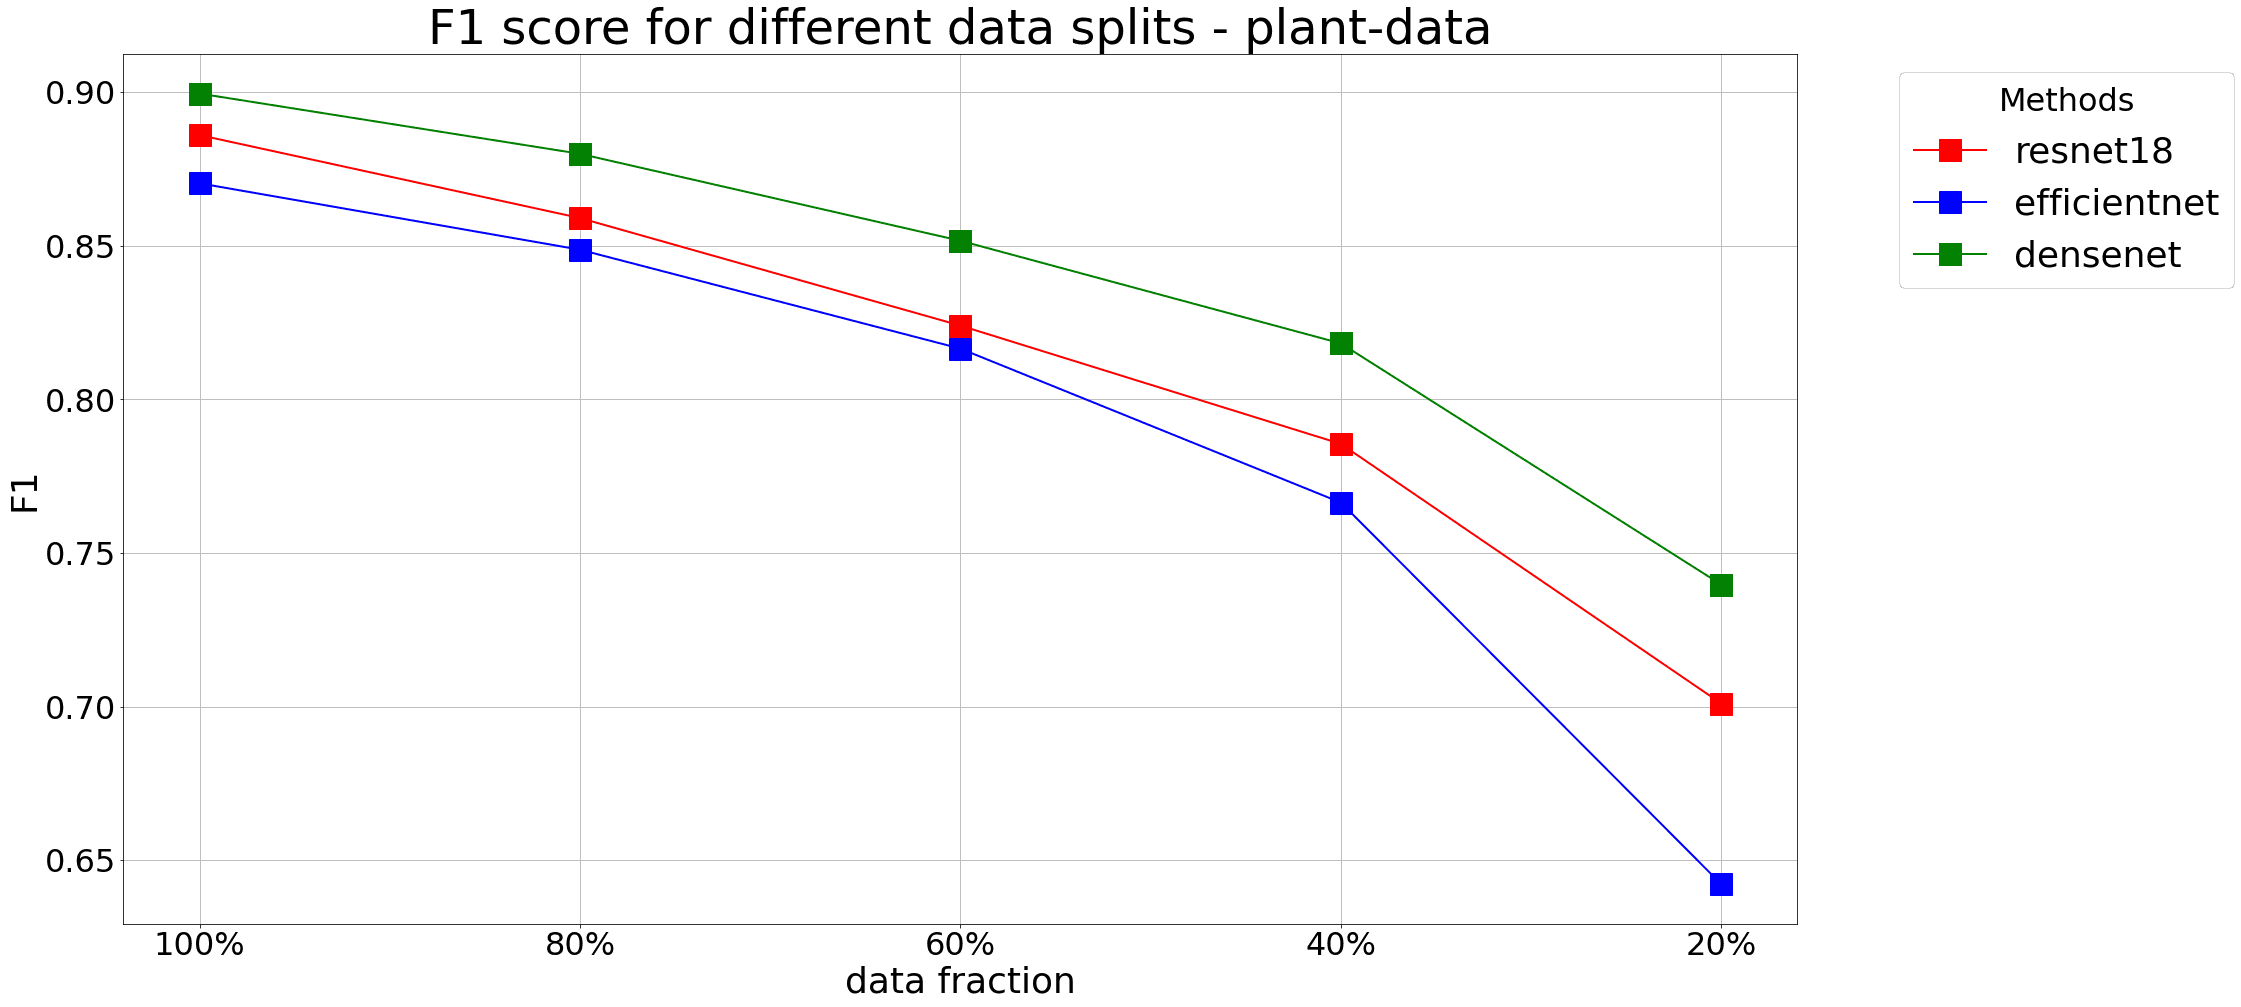
\includegraphics[width=\textwidth]{experiments/models/plant-data-f1.png}
    \caption{Plants dataset, F1 scores}\label{fig:model-scores-plants}
\end{subfigure}

 \caption{F1 scores achieved by models. Each model was trained using a different fraction of the train dataset and then tested on the full test dataset. We can see a significant drop in the models' performance in most of the datasets. The only outliers are visible in models trained on the \textit{Marvel Heroes} dataset (Fig. \ref{fig:model-scores-marvel}), where scores achieved by the models trained on less data are better in two cases.}\label{fig:model-scores}
\end{figure}

\vspace{\baselineskip}

The results of the training process are aligned with the assumption made (remark \ref{remark:performance-drop-while-train}). Models' performance drops with removing more and more data from the training dataset. There are three exceptions, and all of them are related to the Marvel dataset (see Fig. \ref{fig:model-scores-marvel}). All the architectures observed a slight increase of models' score when were trained on less than $100\%$ of the training dataset. That increase did not last when more data was removed, and the rest of the datasets (Fig. \ref{fig:model-scores-dogs}, Fig. \ref{fig:model-scores-food101}, Fig. \ref{fig:model-scores-edible-plants}, Fig. \ref{fig:model-scores-plants}) did not experience the same phenomenon. Detail results are available in appendix \ref{appendix:models:scores}.
\section{Augmentations}\label{section:augmentation}

To simulate real-world scenarios when evaluating attribution methods on datasets, this work uses the multiple augmentations technique. All described augmentations happen only when the calculation of the SSIM metric is done and never influences the results of the \textit{Infidelity} and the \textit{Sensitivity} measures. 

\begin{wrapfigure}{l}{0.45\textwidth}
  \setlength{\belowcaptionskip}{-62pt}
  \centering
  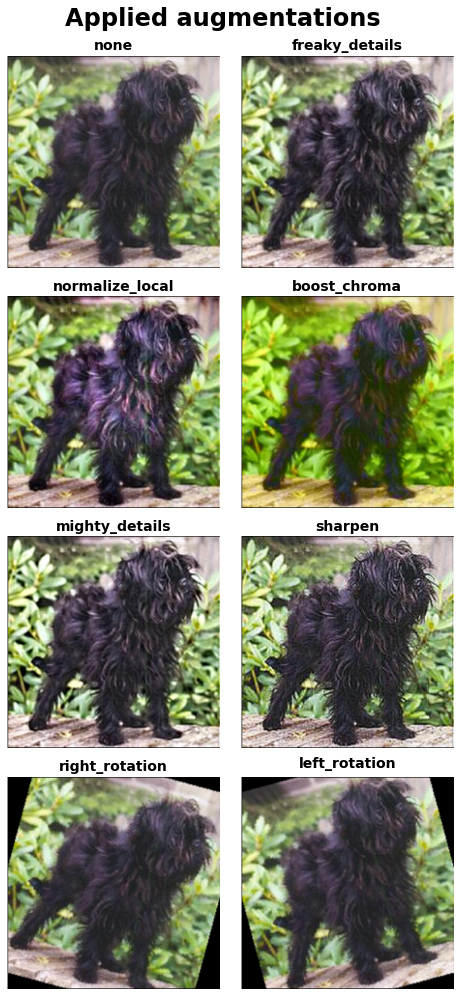
\includegraphics[width=0.40\textwidth]{experiments/aug/augmentations_example.png}
  \caption{Examples  of  real-world augmentations applied on the input image. Image source: \textit{Stanford Dogs} \cite{stanford-dogs}}\label{fig:augmentation-example}
\end{wrapfigure}\leavevmode

\subsection*{Rotation}\label{section:rotations}

This type of augmentation is one of the simplest augmentations we can apply to any image. It uses the rotation matrix\footnote{Rotation matrix is defined as ${\displaystyle R(\theta )={\begin{bmatrix}\cos \theta &-\sin \theta \\\sin \theta &\cos \theta \\\end{bmatrix}}}$ for a two-dimensional vector, where $\theta$ is an angle we want to rotate} to rotate the position of every pixel and fills the empty space with black pixels. This work is using four rotations \textit{\{$-30^{\circ}$ ,$-15^{\circ}$ ,$15^{\circ}$ ,$30^{\circ}$\}} degrees. Because rotation influences the position of the object on the image, when calculating the SSIM value between two attributions, the same rotation is applied to the attribution of the original image. The result of the applied rotation of $15^{\circ}$ and $-15^{\circ}$ can be seen in Figure \ref{fig:augmentation-example} (bottom row).

\subsection*{Freaky Details}

Freaky details filter \cite{freaky_details} is a method used to enhance details of the input image. It works by creating a copy of the image with inverted color and applying a Bilateral filter \cite{tomasi1998bilateral} to it. After the filter, two images are blended together with a \textit{Vivid Light} mode which blends images base on how "light" is a given pixel. It lightens the pixels that are lighter than 50\% gray color and darkens the pixels that are darker than 50\% gray color. The result of the applied filter can be seen in Figure \ref{fig:augmentation-example} in column 2, row 1. It can be applied iteratively, but for the purpose of experiments, it is only applied once. 

\subsection*{Normalize Local}

Local Normalization filter \cite{normalize_local} is a filter that uses local mean and variance to correct local illumination or shading artifacts. For every pixel at the $(x,y)$ position, we normalize its value:

\begin{equation}
    j_{x,y} = \frac{i_{x,y} - \mu_{loc}(i_{x,y})}{\sigma_{loc}(i_{x,y})}
    \label{eq:local-norm-pixel}
\end{equation}

Where $i_{x,y}$ is a value of the pixel at $(x,y)$ position, $\mu_{loc}$ is a mean value of pixels within a given radius, $\sigma_{loc}$ is a variance of the pixels within a given radius. The radius is a parameter, and in the rest of the experiments, it is always $10$ pixels.

\subsection*{Boost Chromaticity}

Boost Chromaticity filter \cite{boost_chroma} is a filter responsible for changing the "colorfulness" of the pixels. It uses the chromaticity diagram to adjust the chromaticity of the pixels. It usually moves the value of the pixel along with the selected color space to avoid spikes on the chromaticity histogram. In the experiments, the $YCbCr$ color space is used.

\subsection*{Mighty Details}

Mighty details filter \cite{mighty_details} is a filter similar to Freaky details. The main difference is that Mighty details apply smoothing (Gaussian blur) before blending two images.

\subsection*{Sharpen}

Sharpening filter \cite{sharpen} is one of the basic filters available in most image processing software. It uses Gaussian blur to create a blurred version of the original image. A blurred image is then compared with the original image, and if the difference between them is greater than a specific threshold, images are subtracted.
\section{Don’t Augment Me}\label{section:dont-augment-me-definition}

The first part of the experiments relies on the hypothesis that real-world augmentations, which do not cause any significant changes in the augmented image and also do not cause a model to change its prediction significantly, may cause an attribution method to produce significantly different attribution of the augmented image. To measure the difference in attributions quantitatively, I am going to use SSIM \cite{wang2004image} metric. Because quantifying a human visual perception cannot be measured with any known metric and is an active field of research, in addition to the SSIM metric, some of the attributions are going to be presented for qualitative measurement.

\subsection*{Procedure}

To be able to calculate the SSIM metric for the attributions, each dataset and method needs to have a maximum range calculated first. This requires an additional run through all images from the dataset through every model and used method to get a maximum value of attribution assigned by a method for a model. This value is used as a data range in SSIM for all attributions using the same method and model. Lists of calculated maximum attribution values are in appendix \ref{appendix:ssim-ranges}. This range is set for a given experiment and not going to be explicitly mentioned in every one of them unless it is relevant to the change in the setup.

\vspace{\baselineskip}

For an image from the test dataset, a set of augmentations will be applied. Augmentations are defined in Section \ref{section:augmentation}, and all of them are used. The original image, as well as augmented images, are then forwarded through a selected model to get a prediction score. If the prediction score of the augmented image is within the $threshold = 0.05$ that of the original image (non-augmented), then the augmented image is accepted for an attribution comparison. To get the attribution, both the augmented image and the original image are forwarded through a selected attribution method, and resulted attributions are the inputs to the SSIM function. The whole process could be defined as:

\begin{equation}
    SSIM_{x, x_i} = \begin{cases} SSIM(A(F, x), A(F, x_i)) & \text{if } |F(x) - F(x_i)| < 0.05 \\ \text{NaN} & \text{otherwise} \end{cases}
\end{equation}

Where $x$ is an original image, $x_i$ is an augmented image, $F$ is a model, $A$ is an attribution method. There is one exception from this equation, and it occurs when the augmentation is a \textit{rotation} (by any angle). The special case includes applying the same rotation to the attribution from the original image and can be summarized as:

\begin{equation}
    SSIM( R(A( F, x ), \theta), A( F, R(x, \theta)) ))
\end{equation}

The main condition ($|F(x) - F(x_i)| < 0.05$) is still in place, the $x_i$ is replaced by the $R(x, \theta)$, which uses a rotation function $R$ and the angle $\theta$. The same rotation $R$ is applied on the result from the attribution method $A( F, x )$. This fixes the issue of calculating the similarity of rotated attribution to the none rotated attribution. This special case is done under the assumption that rotation of the input image should cause the a similar rotation of the attribution for this image. Comparing attribution from the rotated image to the attribution from the original image would not make sense because the region which is the most important for a prediction is rotated by the $\theta$ angle.

\vspace{\baselineskip}

With all SSIM values calculated, each method will have a mean and the standard deviation value calculated. Additionally, mean and standard deviation values will also be calculated per augmentation. The first calculation should allow comparing the methods, and the second is going to be a supplementary check if there are any exceptions for particular augmentation. The qualitative comparison of the results will include visual rendering of selected examples (original images) along with all augmentations applied to that example. Because the amount of augmentations is far greater than it can be displayed in a comprehensive way, augmentations are going to be split into \textit{rotations} and \textit{filters}. \textit{Rotations} will include all available rotations \ref{section:rotations} (4 in total), and \textit{filters} will include everything except the \textit{rotations} (5 in total). For an example to be considered a valid example, all augmented versions of that example have to achieve class score within the $threshold < 0.05$ from the a score of the original image (non-augmented). This is a more restrictive criterion than the one used for each augmentation separately but removes any potential misinformation on which augmentation is used for valid or not.

\section{Can I Rely On You}\label{section:can-i-rely-on-you-definition}

The second part of the experiments is focused on testing the hypothesis that two of the most popular measures of XAI methods are not reliable when trying to use them to compare methods even within the same data domain. To be able to check if that hypothesis is true, we need to define how the measure should behave for it to be considered reliable.

\begin{definition}\label{def:reliability}
    Given an XAI method $A_1$ and $A_2$ and the measure $S(A)$, measure $S$ is considered reliable, when within the same data domain and model architecture, measures calculated for method $A_1$ always have the same relation to the measures calculated for the method $A_2$.
\end{definition}

\begin{figure}[h]
  \centering
 \begin{subfigure}{.3\textwidth}
    \centering
    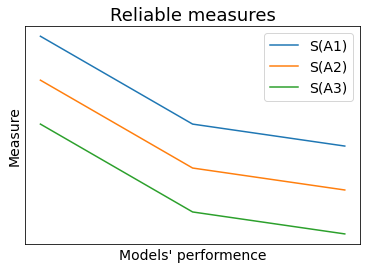
\includegraphics[width=\textwidth]{experiments/desc/rel1.png}
    \caption{}\label{fig:rel-measure-1}
\end{subfigure}
 \begin{subfigure}{.3\textwidth}
    \centering
    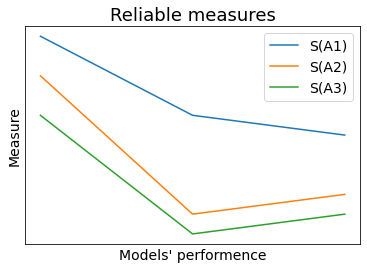
\includegraphics[width=\textwidth]{experiments/desc/rel2.png}
    \caption{}\label{fig:rel-measure-2}
\end{subfigure}
 \begin{subfigure}{.3\textwidth}
    \centering
    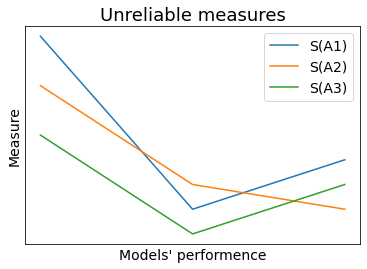
\includegraphics[width=\textwidth]{experiments/desc/unrel1.png}
    \caption{}\label{fig:unrel-measure}
\end{subfigure}

 \caption{An example of reliable measures (Fig. \ref{fig:rel-measure-1}, \ref{fig:rel-measure-2}) and unreliable measures (Fig. \ref{fig:unrel-measure})}\label{fig:reliable-measures-example}
\end{figure}

To illustrate definition \ref{def:reliability}, let us consider an example in Figure \ref{fig:reliable-measures-example}. Each chart represents a relation between the measure score and the models' performance (it could be $F1$ or any valid metric). The ideal measure is shown in Figure \ref{fig:rel-measure-1}, where the relation between values for different attribution methods ($A1$, $A2$, and $A3$) remain the same with the change of models' performance. Changes in the absolute value are not relevant here. The second example (Fig. \ref{fig:rel-measure-2}) is also a valid measure but not as ideal as the first one. Relation between values is changed, but the order of the values is always the same. The third example (Fig. \ref{fig:unrel-measure}) shows the behavior of the unreliable method. The relation between values is changing, and the order in which values for each method are presented is also changing. If there were only two methods in the third example ($A1$ and $A3$), we could assume the measure is reliable. That is the reason why when testing a given measure, we should use more data points.

\subsection*{Procedure}

To properly validate measure Infidelity (Section: \ref{section:infidelity}) and Sensitivity (Section: \ref{section:sensitivity}), each of them has to be tested on every trained model. That gives a total of $375$ different data points for the measure (5 XAI methods $\times$ 5 datasets $\times$ 5 train data fractions $\times$ 3 models). Each data point consists of measures for every sample from the train dataset used for a particular model.

\begin{remark}
The Integrated Gradients (Section \ref{section:ig}) method is not used in this experiment because computing the value of Sensitivity for this method requires more than 11GB of memory.
\end{remark}

Infidelity uses a Gaussian noise with a $\mu = 0$ and $\sigma = 0.003$ to perturb images. Sensitivity creates $10$ perturbed images with the help of the function that samples uniformly random from the $L_{Infinity}$ ball with $0.02$ radius. The results from each data point are processed, and the mean and standard deviation values are calculated. 